\newpage
\section{Анализ предметной области}
\subsection{Концептуальная модель предметной области}

Определим основные объекты предметной области и выясним отношения между ними.

\subsubsection{Пациент}
Сущность отражает личную информацию о реальном пациенте.

Атрибуты:
\begin{enumerate}
  \item паспортные данные;
  \item номер полиса;
  \item номер личной больничной карты\footnote{
  	Сложно будет перевести сразу все учреждение на электронные больничные карты
  	поэтому некоторое время обычная больничная карта и электронная будут
  	сущестовать параллельно.
  };
  \item контактные данные.
\end{enumerate}

\subsubsection{Врач}
Сущность отражает данные о реальном докторе.

Атрибуты:
\begin{enumerate}
  \item паспортные данные;
  \item контактные данные;
  \item профессиональные данные; 
\end{enumerate}

\subsubsection{Менеджер}
Сущность отражает человека контролирующего работу системы.

Атрибуты:
\begin{enumerate}
  \item паспортные данные;
  \item контактные данные;
  \item профессиональные данные.   
\end{enumerate}

\subsubsection{Диагноз}
Сущность отражает реальный диагноз согласно “Международной статистической
классификации болезней и проблем, связанных со здоровьем” (ICD 10).

Атрибуты:
\begin{enumerate}
  \item класс диагноза;
  \item название диагноза.   
\end{enumerate}

\subsubsection{Лекарство}
Сущность отражает реальное лекарственный препарат.

Атрибуты:
\begin{enumerate}
  \item название лекарства;
  \item побочные эффекты;
  \item время приема;
  \item дозы;
  \item порядок приема. 
\end{enumerate}

\subsubsection{Обследование}
Сущность отражает реальное обследование доступное пациентам лечащего учреждения
в процессе лечения.

Атрибуты:
\begin{enumerate}
  \item суть обследования; 
  \item дата обследования; 
  \item результат обследования. 
\end{enumerate}

\subsubsection{Прием}
Сущность отражает реальный прием у врача. Так как система должна иметь
возможноть сопровождать два типа приема: обычный и интернет прием, необходимо
чтобы набор атрибутов у них был максимально одинаковым. Выполнение данного
условия облегчит перевод учреждения на электронный прием.
 
Атрибуты:
\begin{enumerate}
  \item дата приема; 
  \item результат приема; 
  \item данные сопровождающие прием. 
\end{enumerate}

\subsubsection{Документ}
Сущность отражает документ, который врач составляет по результатам медицинского
приема. Доступ к документу должен быть только у пациента, на которого составлен
данный документ и у его лечащего врача, так как это медицинская информация.
Атрибуты:
\begin{enumerate}
  \item время создания документа;
  \item сдержащаяся информация. 
\end{enumerate}

\begin{figure}[h]
\center{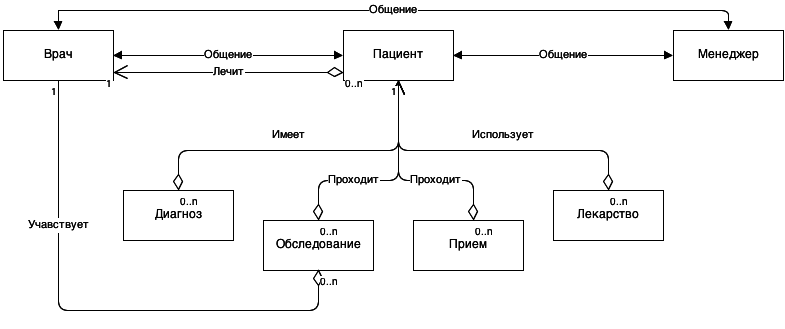
\includegraphics[width=1\linewidth]{object_model.eps}}
\caption{Связи между объектами предметной области}
\label{ris:object_model}
\end{figure}

Выявленные объекты предметной области (рисунок \ref{ris:object_model}), не покрывают всех
функциональных требований к системе и не учитывают технических реализаций и алгоритмов
построения информационных систем.

\subsection{Уточненние объектов предметной области}
Объекты “Врач”, “Пациент” и “Менеджер” имеют общий набор атрибутов, который
логично вынести в отдельный объект родитель “Пользователь”. Данный шаг упростит
процедуры регистрации, авторизации и процесс контроля прав доступа к системе,
так как необходимо будет контролировать только один объект вместо трех.

Объекты “Прием” и “Обследование” - это некоторые события. Логичным будет
выделить отдельный объект родитель - “Событие”. “Событие” будет связано с
пользователем через объект “Календарь” - отражающий определенный этап лечения.
Каждое событие имеет “Результат”. Событие может быть повторяющимся (прием
лекарственного препарата 3 раза в день). 

Лекарственные препараты и диагнозы являются справочниками, которые логичным
будет наследовать от объекта родителя “Справочник”.

“Справочник” и “Электронная карта” - это документы. Для облегчения работы с ними
логичным будет ввести объект родитель “Документ”.

На рисунке \ref{ris:data_logic_model} изображена уточненная модель предметной
области.
 
\begin{figure}[h]
\center{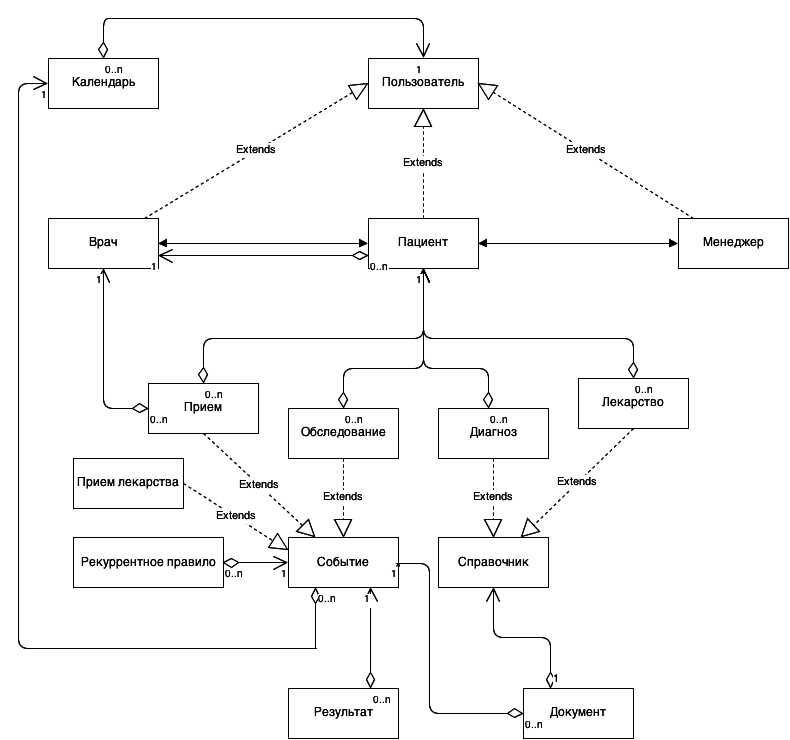
\includegraphics[width=1\linewidth]{data_logic_model.eps}}
\caption{Уточненная модель предметной области}
\label{ris:data_logic_model}
\end{figure}